% This is the Reed College LaTeX thesis template. Most of the work
% for the document class was done by Sam Noble (SN), as well as this
% template. Later comments etc. by Ben Salzberg (BTS). Additional
% restructuring and APA support by Jess Youngberg (JY).
% Your comments and suggestions are more than welcome; please email
% them to cus@reed.edu
%
% See http://web.reed.edu/cis/help/latex.html for help. There are a
% great bunch of help pages there, with notes on
% getting started, bibtex, etc. Go there and read it if you're not
% already familiar with LaTeX.
%
% Any line that starts with a percent symbol is a comment.
% They won't show up in the document, and are useful for notes
% to yourself and explaining commands.
% Commenting also removes a line from the document;
% very handy for troubleshooting problems. -BTS

% As far as I know, this follows the requirements laid out in
% the 2002-2003 Senior Handbook. Ask a librarian to check the
% document before binding. -SN

%%
%% Preamble
%%
% \documentclass{<something>} must begin each LaTeX document
\documentclass[12pt,twoside]{reedthesis}
% Packages are extensions to the basic LaTeX functions. Whatever you
% want to typeset, there is probably a package out there for it.
% Chemistry (chemtex), screenplays, you name it.
% Check out CTAN to see: http://www.ctan.org/
%%
\usepackage{graphicx,latexsym}
\usepackage{amsmath}
\usepackage{amssymb,amsthm}
\usepackage{longtable,booktabs,setspace}
\usepackage{chemarr} %% Useful for one reaction arrow, useless if you're not a chem major
\usepackage[hyphens]{url}
% Added by CII
\usepackage{hyperref}
\usepackage{lmodern}
\usepackage{float}
\floatplacement{figure}{H}
% End of CII addition
\usepackage{rotating}

% Next line commented out by CII
%%% \usepackage{natbib}
% Comment out the natbib line above and uncomment the following two lines to use the new
% biblatex-chicago style, for Chicago A. Also make some changes at the end where the
% bibliography is included.
%\usepackage{biblatex-chicago}
%\bibliography{thesis}


% Added by CII (Thanks, Hadley!)
% Use ref for internal links
\renewcommand{\hyperref}[2][???]{\autoref{#1}}
\def\chapterautorefname{Chapter}
\def\sectionautorefname{Section}
\def\subsectionautorefname{Subsection}
% End of CII addition

% Added by CII
\usepackage{caption}
\captionsetup{width=5in}
% End of CII addition

% \usepackage{times} % other fonts are available like times, bookman, charter, palatino

% Syntax highlighting #22

% To pass between YAML and LaTeX the dollar signs are added by CII
\title{Pronouns Good or Bad: Attitudes and Relationships with Gendered Pronouns in Gender-Diverse Undergraduates}
\author{Jade Fung}
% The month and year that you submit your FINAL draft TO THE LIBRARY (May or December)
\date{May 2020}
\division{Philosophy, Religion, Psychology, and Linguistics}
\advisor{Vasiliy Safin}
\institution{Reed College}
\degree{Bachelor of Arts}
%If you have two advisors for some reason, you can use the following
% Uncommented out by CII
% End of CII addition

%%% Remember to use the correct department!
\department{Psychology}
% if you're writing a thesis in an interdisciplinary major,
% uncomment the line below and change the text as appropriate.
% check the Senior Handbook if unsure.
%\thedivisionof{The Established Interdisciplinary Committee for}
% if you want the approval page to say "Approved for the Committee",
% uncomment the next line
%\approvedforthe{Committee}

% Added by CII
%%% Copied from knitr
%% maxwidth is the original width if it's less than linewidth
%% otherwise use linewidth (to make sure the graphics do not exceed the margin)
\makeatletter
\def\maxwidth{ %
  \ifdim\Gin@nat@width>\linewidth
    \linewidth
  \else
    \Gin@nat@width
  \fi
}
\makeatother

%Added by @MyKo101, code provided by @GerbrichFerdinands
\newlength{\cslhangindent}
\setlength{\cslhangindent}{1.5em}
\newenvironment{cslreferences}%
  {\setlength{\parindent}{0pt}%
  \everypar{\setlength{\hangindent}{\cslhangindent}}\ignorespaces}%
  {\par}

\renewcommand{\contentsname}{Table of Contents}
% End of CII addition

\setlength{\parskip}{0pt}

% Added by CII

\providecommand{\tightlist}{%
  \setlength{\itemsep}{0pt}\setlength{\parskip}{0pt}}

\Acknowledgements{

}

\Dedication{

}

\Preface{

}

\Abstract{

}

	\usepackage{float}
 \floatplacement{figure}{H}
	\usepackage{booktabs}
 \usepackage{longtable}
 \usepackage{array}
 \usepackage{multirow}
 \usepackage{wrapfig}
 \usepackage{float}
 \usepackage{colortbl}
 \usepackage{pdflscape}
 \usepackage{tabu}
 \usepackage{threeparttable}
 \usepackage{threeparttablex}
 \usepackage[normalem]{ulem}
 \usepackage{makecell}
 \usepackage{xcolor}
% End of CII addition
%%
%% End Preamble
%%
%
\begin{document}

% Everything below added by CII
  \maketitle

\frontmatter % this stuff will be roman-numbered
\pagestyle{empty} % this removes page numbers from the frontmatter



  \hypersetup{linkcolor=black}
  \setcounter{tocdepth}{2}
  \tableofcontents

  \listoftables

  \listoffigures



\mainmatter % here the regular arabic numbering starts
\pagestyle{fancyplain} % turns page numbering back on

\hypertarget{introduction}{%
\chapter*{Introduction}\label{introduction}}
\addcontentsline{toc}{chapter}{Introduction}

Hello and welcome to my thesis. This will very much be an active document until at least May 1st, when it will be due. Join me as I write about pronouns :-)

\hypertarget{literature-review}{%
\chapter{Literature Review}\label{literature-review}}

Let's review: gendered pronouns.

\hypertarget{methods}{%
\chapter{Methods}\label{methods}}

\hypertarget{participants}{%
\section{Participants}\label{participants}}

Undergraduate students from Reed College in Portland, Oregon participated in an online survey about ``attitudes towards gendered pronouns.'' Participants were recruited through online advertisements and posters around campus.

Participants of all genders were recruited, including cisgender participants. Tate, Youssef, \& Bettergarcia (2014) advocate for the integration of cisgender and non-cisgender gender research into one body of research on gender identity development. They push back on the common assumption that cisgender people do not undergo a period of self-reflection and self-categorization in the maturation of their gender identity. Furthermore, by not excluding cisgender participants from the study, we allowed freer self-categorization e.g.~for the inclusion of people who identified as cisgender and non-binary. Therefore, there were virtually no exclusion criteria for participation. Advertisements included text such as ``Hey! Do you use pronouns and/or have a gender?'' in an attempt to reach as many people as possible.

607 people responded to the survey. 117 responses were excluded because they were incomplete. 13 were excluded because they were not undergraduate students. Our final sample was 477 students. Notably, Reed's undergraduate student body size is 1,457 students (Reed College Institutional Research, 2019), so this sample includes 33\% of the school.

\hypertarget{survey}{%
\section{Survey}\label{survey}}

Participants participated online through Qualtrics. The survey was advertised as taking 5-10 minutes. Participants agreed to a consent page, then answered questions about their relationship with pronouns and gender, then questions about misgendering frequency (McLemore, 2015), then the Transgender Inclusive Behavior Scale (Kattari, O'Connor, \& Kattari, 2018), then the Transgender Congruence Scale (Kozee, Tylka, \& Bauerband, 2012), and the finally questions about their demographics.

\hypertarget{gendered-pronoun-attitude-survey-gpas}{%
\subsection{Gendered Pronoun Attitude Survey (GPAS)}\label{gendered-pronoun-attitude-survey-gpas}}

The GPAS was developed as a broad survey of undergraduate students' relationships and experiences with gendered pronouns. Many items were phrased similarly to questions from the TCS. However, as this is a very novel area of study, the author created most of them herself in consultation with other gender-diverse peers.

Responses were collected as five-point likert scales ranging from ``Strongly Disagree'' to ``Strongly Agree.'' In the first block of questions, participants were asked to report their experiences from the past two weeks. This was done to reflect the Transgender Congruence Scale (TCS) by Kozee et al. (2012). The TCS asked participants to reflect on their relationship with gender in the past two weeks. Participants were given definitions for gender identity and pronouns: \emph{Gender identity is defined as the gender/genders that you experience yourself as; it is not necessarily related to your assigned gender at birth. Pronouns are the words someone else can use to refer to you. For example, someone who uses she/her pronouns would be referred to like this: ``She rides the bus.''}
\begin{table}

\caption{\label{tab:unnamed-chunk-1}Pronoun attitude questionnaire items: past 2 weeks}
\centering
\begin{tabular}[t]{l}
\hline
Item Description\\
\hline
I feel comfortable sharing my pronouns in most settings.\\
\hline
I feel comfortable sharing my pronouns in non-academic settings in the Reed community.\\
\hline
I feel comfortable sharing my pronouns in classes at Reed.\\
\hline
I want to share my pronouns in most settings.\\
\hline
I want to share my pronouns in non- academic settings in the Reed community.\\
\hline
I want to share my pronouns in classes at Reed.\\
\hline
I feel more comfortable sharing my pronouns if I am with people who may have similar gender identities to me.\\
\hline
I feel more comfortable introducing myself with my pronouns if someone else does first.\\
\hline
I feel more comfortable introducing myself with my pronouns in class if the professor does first.\\
\hline
I am concerned that sharing my pronouns will draw unwanted attention to myself in most settings.\\
\hline
I am concerned that sharing my pronouns will draw unwanted attention to myself in non-academic settings in the Reed community\\
\hline
I am concerned that sharing my pronouns will draw unwanted attention to myself in class at Reed.\\
\hline
I feel that the gender that people perceive me as and my pronouns are consistent with one another.\\
\hline
I feel that my internal gender identity and pronouns are consistent with one another.\\
\hline
I feel that my pronouns represent my gender identity well.\\
\hline
If I don’t tell people what my pronouns are, they will misgender me.\\
\hline
I don’t need to tell people what my pronouns are, because they usually assume correctly.\\
\hline
I feel like people understand me better when I share my pronouns.\\
\hline
\end{tabular}
\end{table}
In the second block of questions, participants were asked to reflect on their experience across their entire time at Reed. These questions drew on participants extended experience at the college and reflection on each semester.
\begin{table}

\caption{\label{tab:unnamed-chunk-2}Pronoun attitude questionnaire items: entire time at Reed}
\centering
\begin{tabular}[t]{l}
\hline
Item Description\\
\hline
In classes at Reed, professors usually introduce themselves with their pronouns\\
\hline
In classes at Reed, students usually introduce themselves with their pronouns\\
\hline
Enough is being done at Reed to support people who have the same gender as me.\\
\hline
\end{tabular}
\end{table}
\hypertarget{transgender-inclusive-behavior-scale-tibs}{%
\subsection{Transgender Inclusive Behavior Scale (TIBS)}\label{transgender-inclusive-behavior-scale-tibs}}

The Transgender Inclusive Behavior Scale was developed by Kattari et al. (2018) to provide a measure for actions and modes of communication that are inclusive and supportive of transgender people. The TIBS was developed for participants of all gender identities---not exclusively cisgender people.

The TIBS includes a broad array of trans affirming behaviors. This includes several items such as sharing their own pronouns and asking for others', educating themselves on local policies that may affect transgender people, and speaking out against transphobia in their communities.

Responses were collected as five-point likert scales ranging from ``Never'' to ``Always.'' Each participant's responses were added to produce a score that generally represented how many inclusive behaviors one performed.

While selecting our measures, we elected to use the TIBS in lieu of a measure such as the transphobia scale developed by Nagoshi et al. (2008). This was done to generally frame the study as positive and affirming for transgender people. Administering questions about transphobic attitudes to transgender people who are the victims of transphobia and transmisogynistic violence could have been significantly more distressing than asking about affirming and supportive behaviors. Essentially, the TIBS was included as a proxy for how intentionally participants supported and affirmed their transgender peers.

An added potential benefit to administering the TIBS to cisgender participants is that it potentially includes actions that cisgender people had not yet considered doing to support their transgender peers. As data collection progressed, the author received several messages from participants reporting that they had never considered some of the actions, like ensuring that gender-neutral bathrooms were available at events that they organized.

\hypertarget{transgender-congruence-scale-tcs}{%
\subsection{Transgender Congruence Scale (TCS)}\label{transgender-congruence-scale-tcs}}

The Transgender Congruence Scale was developed by Kozee et al. (2012) to provide a measure for how transgender people feel ``genuine, authentic, and comfortable with their gender identity and external appearance.'' The TCS was developed for transgender participants. However, we elected to administer the TCS to cisgender participants as well. This was done to avoid presuming that cisgender people have a purely passive relationship with their gender, as is advocated for by Tate et al. (2014).

Responses were collected as five-point likert scales ranging from ``Strongly Disagree'' to ``Strongly Agree'' Each participant's responses were added to produce a score that generally represented how congruent one felt with one's gender identity. The TCS consists of 12 items that include relationships between the participant's gender identity, their physical appearance and presentation, their body, and their social experience with gender.

\hypertarget{demographic-quesitons}{%
\subsection{Demographic Quesitons}\label{demographic-quesitons}}

Participants were asked their age, ethnicity, year at Reed, major, gender, pronouns, and sexual orientation. Sexual orientation and pronouns were short answer write-in field. This was done to avoid presupposing any orientation or pronoun over the other, as well as to allow participants to describe their relationship with either in as much or as little depth as they deemed fit.

Gender was collected in four parts: first, participants responded to a short answer write-in field. Then, they answered three yes/no questions: ``Are you cisgender?'', ``Are you transgender?'', and ``Is your gender non-binary?''. Answering yes on one question did not force participants to answer no on any others. By separating cisness, transness, and non-binary status from gender identity, we allowed these words to serve as modes of relating to one's gender. Because this is a study of gender identity and trans experiences, it was analytically important to separate \emph{relationship} to gender identity from gender identity. However, in everyday life, the author firmly believes that this does not matter, e.g.~there is no fundamental difference between cisgender and transgender women, and to treat them any differently is to perpetuate transmisogynistic violence.

\hypertarget{results}{%
\chapter{Results}\label{results}}

\hypertarget{demographics}{%
\section{Demographics}\label{demographics}}

\hypertarget{gender}{%
\subsection{Gender}\label{gender}}

I collected gender-related demographic data by asking participants to write in their gender identity and answer a series of yes/no questions: ``Are you cisgender?,'' ``Are you transgender?,'' and ``Is your gender non-binary?'' Answering yes on one question did not force the participants to answer no on others---this treated gender identity as a collection of separate, related labels that participants may or may not identify with simultaneously. Responses for the write-in question were qualitatively coded by me.

Overall, 317 participants identified as cisgender, 81 identified as transgender, and 141 identified their gender as non-binary. It is important to note that there is overlap among these groups. 63 participants said they were transgender and non-binary, 16 participants said they were cisgender and non-binary, and 1 participant said they were cisgender, transgender, and non-binary.

Qualitative themes were decided by the author after examining the data and consulting with a number of gender-diverse peers. The most commonly occuring themes were woman (\emph{N} = 220), man (\emph{N} = 120), non-binary (\emph{N} = 94), cisgender (\emph{N} = 36), transgender (\emph{N} = 26), questioning (\emph{N} = 24), masculine (\emph{N} = 18), agender (\emph{N} = 15), genderfluid (\emph{N} = 15), and queer (\emph{N} = 8).

For the purposes of analysis, seven \emph{artificial} gender groups were created: cisgender man, cisgender woman, transgender man, transgender woman, cisgender non-binary person, non-binary person, and transgender non-binary person. It is important to note that these bins are artificial and are not representative of each individual's own gender and experience. For example, ``non-binary'' can have many meanings and is best understood as an umbrella term that encompasses many genders, including individuals who's gender is just ``non-binary.''
\begin{table}

\caption{\label{tab:unnamed-chunk-3}Artificial gender bins created for the purpose of analysis.}
\centering
\begin{tabular}[t]{l|r}
\hline
Gender Bin & N\\
\hline
Cis Woman & 182\\
\hline
Cis Man & 101\\
\hline
Non-binary & 80\\
\hline
Trans Non-binary & 48\\
\hline
Trans Woman & 20\\
\hline
Cis Non-binary & 15\\
\hline
Trans Man & 12\\
\hline
\end{tabular}
\end{table}
The cisgender man and cisgender woman groups include all participants that only indicated that they were cisgender and indicated that they were a man or woman in the write-in gender field. The transgender man and transgender woman groups were the same as the cisgender groups, but included participants who indicated that they were transgender.

The cisgender non-binary group includes all participants who indicated that they were cisgender and non-binary. This group includes cisgender non-binary men and cisgender non-binary women. The non-binary group includes all participants that only indicated that they were non-binary, as well as participants who indicated that they were neither cisgender nor transgender. This group includes non-binary men and non-binary women. The transgender non-binary group includes all participants that indicated that they were non-binary and transgender. This group includes transgender non-binary men and transgender non-binary women.

\hypertarget{pronouns}{%
\subsection{Pronouns}\label{pronouns}}

Participants were asked their pronouns in a write-in box. Pronouns were qualitatively coded by the author. No participants reported using any other pronouns besides he/him, she/her, and they/them. However, many participants reported using multiple pronouns. It should be noted that individuals that use multiple pronouns may prefer one over the other, or use different pronouns in specific situations. This is not reflected in these data.
\begin{table}

\caption{\label{tab:cockandballs}Participant pronouns}
\centering
\begin{tabular}[t]{l|r}
\hline
Pronouns & N\\
\hline
she/her & 199\\
\hline
he/him & 127\\
\hline
they/them & 65\\
\hline
she/her \& they/them & 35\\
\hline
he/him \& they/them & 19\\
\hline
all pronouns & 10\\
\hline
he/him \& she/her & 2\\
\hline
\end{tabular}
\end{table}
The most common gender and pronoun combinations were cisgender women that used she/her, (\emph{N} = 175), cisgender men that used he/him, (\emph{N} = 96), transgender non-binary people that used they/them, (\emph{N} = 32), non-binary people that used they/them, (\emph{N} = 28), non-binary people that used she/her and they/them, (\emph{N} = 16), trans men that used he/him, (\emph{N} = 12), and trans women that used she/her, (\emph{N} = 11).

\hypertarget{sexuality}{%
\subsection{Sexuality}\label{sexuality}}

Participants were asked to report their sexuality in a write-in field. Responses were qualitatively coded by the author. Many responses were coded with multiple themes, so the total \emph{N} exceeds the sample size. One exceptionally common response was ``bisexual/pansexual,'' (\emph{N} = 11), which was coded with both themes.
\begin{table}

\caption{\label{tab:unnamed-chunk-4}Participant sexuality}
\centering
\begin{tabular}[t]{l|r}
\hline
Sexuality & N\\
\hline
Bisexual & 178\\
\hline
Straight & 115\\
\hline
Pansexual & 49\\
\hline
Queer & 40\\
\hline
Questioning & 39\\
\hline
Gay & 35\\
\hline
Lesbian & 35\\
\hline
Asexual & 16\\
\hline
Aspec & 15\\
\hline
\end{tabular}
\end{table}
The most common gender and sexualities were bisexual cisgender women, (\emph{N} = 70), straight cisgender men, (\emph{N} = 56), straight cisgender women, (\emph{N} = 50), bisexual non-binary people, (\emph{N} = 33), bisexual cisgender men, (\emph{N} = 26), and bisexual transgender non-binary people, (\emph{N} = 23).

\hypertarget{experiences-with-misgendering}{%
\section{Experiences with Misgendering}\label{experiences-with-misgendering}}

Similar to McLemore (2015), we had participants report how frequently they were misgendered and how stigmatized misgendering made them feel. However, unlike McLemore (2015), we administered these questions to cisgender people as well. Independent t-tests were used to compare the cisgender and non-cisgender participants. Non-cisgender participants (\emph{M} = 3.28, \emph{SD} = 0.96) reported being misgendered more frequently than cisgender participants (\emph{M} = 1.45, \emph{SD} = 1.45), \emph{t}(230.94) = 21.6, \emph{p} \textless{} 0.001.
Non-cisgender participants (\emph{M} = 3.15, \emph{SD} = 1.3) also reported feeling more stigmatized when misgendered than than cisgender participants (\emph{M} = 1.59, \emph{SD} = 1.59), \emph{t}(261.06) = 12.9, \emph{p} \textless{} 0.001.
\begin{table}

\caption{\label{tab:unnamed-chunk-5}Misgendering frequency for non-cisgender and cisgender participants}
\centering
\begin{tabular}[t]{l|r|r}
\hline
“How often do people ‘misgender’ you?” & Non-cisgender (\%) & Cisgender (\%)\\
\hline
Never & 6.4 & 68.8\\
\hline
Rarely & 14.0 & 24.9\\
\hline
Sometimes & 30.6 & 4.7\\
\hline
Often & 44.6 & 1.3\\
\hline
Always & 4.5 & 0.3\\
\hline
\end{tabular}
\end{table}
\begin{table}

\caption{\label{tab:unnamed-chunk-6}Felt stigma when misgendered for non-cisgender and cisgender participants}
\centering
\begin{tabular}[t]{l|r|r}
\hline
“I feel stigmatized (...) when I am misgendered.” & Non-cisgender (\%) & Cisgender (\%)\\
\hline
Not at all & 12.2 & 68.5\\
\hline
Slightly & 20.5 & 12.0\\
\hline
Somewhat & 28.2 & 13.4\\
\hline
Considerably & 18.6 & 4.0\\
\hline
Very & 20.5 & 2.2\\
\hline
\end{tabular}
\end{table}
Pearson's Chi-squared tests were used to compare the misgendering frequency observed in McLemore (2015) to the non-cisgender participants in the present study.
There were significant differences when compared to both the study 1 population, \emph{X2} (4, \emph{N} = 864) = 178.18, \emph{p} = 0, and the study 2 population, \emph{X2} (4, \emph{N} = 902) = 228.69, \emph{p} = 0.

We performed a one-way ANOVA examining gender and pronouns' effect on misgendering frequency and felt stigma. There was a significant effect of gender, \emph{F}(6, 428) = 131.73, \emph{p} \textless{} 0.001, and pronouns, \emph{F}(6, 428) = 12.53, \emph{p} \textless{} 0.001, on misgendering frequency. A post-hoc Tukey test revealed that cis men, (\emph{M} = 1.3, \emph{SD} = 0.5), and cis women, (\emph{M} = 1.36, \emph{SD} = 0.62), get misgendered less frequently than trans men, (\emph{M} = 3.25, \emph{SD} = 0.87), trans women, (\emph{M} = 3.5, \emph{SD} = 0.95), cis non-binary people, (\emph{M} = 2.07, \emph{SD} = 1.28), non-binary people, (\emph{M} = 3.03, \emph{SD} = 1.06), and trans non-binary people, (\emph{M} = 3.56, \emph{SD} = 0.77). Cis non-binary people also get misgendered less than trans men men, trans women, non-binary people, and trans non-binary people. Trans non-binary people also get misgendered more than non-binary people. Additionally, people who use they/them pronouns, (\emph{M} = 3.71, \emph{SD} = 0.82), get misgendered more than people who use he/him pronouns, (\emph{M} = 1.6, \emph{SD} = 0.94), she/her pronouns, (\emph{M} = 1.48, \emph{SD} = 0.79), both he/him and they/them pronouns, (\emph{M} = 2.84, \emph{SD} = 1.01), and both she/her and they/them pronouns, (\emph{M} = 2.66, \emph{SD} = 1.08).

There was also a significant effect of gender, \emph{F}(6, 389) = 43.4, \emph{p} \textless{} 0.001, but not of pronouns, \emph{F}(6, 389) = 0.74, \emph{p} = 0.61, on felt stigma when misgendered. A post-hoc Tukey test revealed that cis men, (\emph{M} = 1.42, \emph{SD} = 0.88), and cis women, (\emph{M} = 1.67, \emph{SD} = 1.05), feel less stigmatized when misgendered than trans men, (\emph{M} = 4.25, \emph{SD} = 0.75), trans women, (\emph{M} = 3.45, \emph{SD} = 1.54), non-binary people, (\emph{M} = 2.59, \emph{SD} = 1.09), and trans non-binary people, (\emph{M} = 3.62, \emph{SD} = 1.23). Cis non-binary people, (\emph{M} = 1.87, \emph{SD} = 0.99), also feel less stigmatized when misgendered than trans men, trans women, and trans non-binary people. Non-binary people also feel less stigmatized when misgendered than trans men and trans non-binary people.

\hypertarget{gender-congruence}{%
\section{Gender Congruence}\label{gender-congruence}}

Kozee et al. (2012) developed the TCS (Transgender Congruence Scale) to measure transgender individuals' relationship and comfort between their inner gender identity, physical appearance, and social experience of gender. In this study, the TCS was administered to cisgender participants as well.

A single sample t-test revealed that non-cisgender participants (\emph{M} = 34.26, \emph{SD} = 5.5) scored lower on the TCS than cisgender participants (\emph{M} = 45.53, \emph{SD} = 6.23), \emph{t}(348.89) = -20.04, \emph{p} \textless{} 0.001.

A one-way ANOVA demonstrated significant effects of gender on TCS scores, \emph{F}(6, 445) = 71.24, \emph{p} \textless{} 0.001. A post-hoc Tukey test revealed that cis men, (\emph{M} = 46.19, \emph{SD} = 5.55), and cis women, (\emph{M} = 45.98, \emph{SD} = 5.8), have significantly higher TCS scores than trans men, (\emph{M} = 36.08, \emph{SD} = 2.84), trans women, (\emph{M} = 35.11, \emph{SD} = 4.12), cis non-binary people, (\emph{M} = 37.93, \emph{SD} = 9.05), non-binary people, (\emph{M} = 33.97, \emph{SD} = 5.89), and trans non-binary people, (\emph{M} = 33.94, \emph{SD} = 5.81).
\begin{figure}
\centering
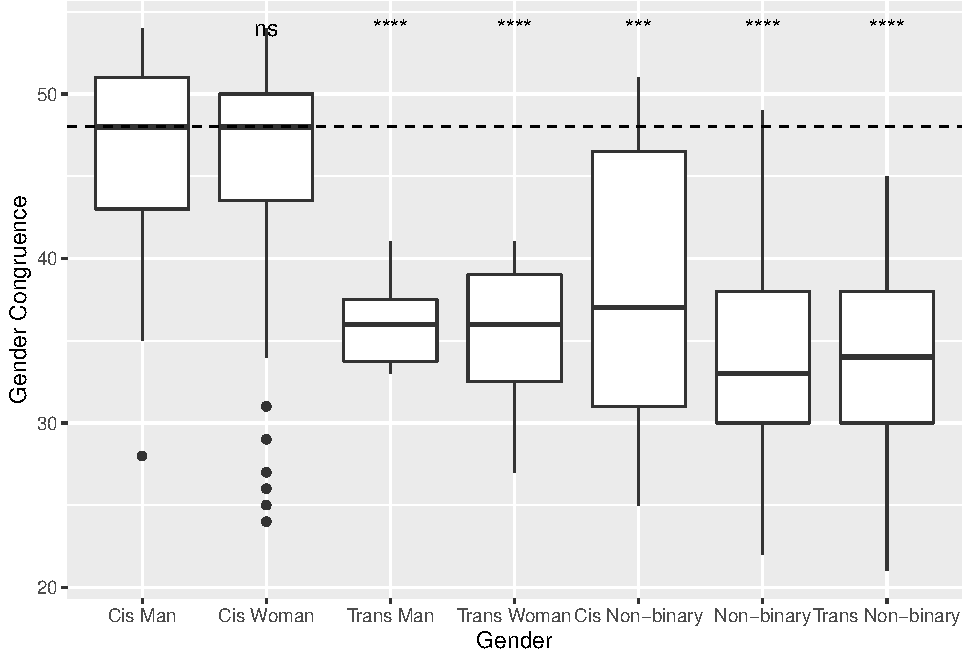
\includegraphics{thesis_files/figure-latex/unnamed-chunk-7-1.pdf}
\caption{\label{fig:unnamed-chunk-7}TCS Scores by Gender}
\end{figure}
\hypertarget{transgender-inclusive-behaviors}{%
\section{Transgender Inclusive Behaviors}\label{transgender-inclusive-behaviors}}

Kattari et al. (2018) developed the Transgender Inclusive Behavior Scale (TIBS) as a method of quantifying the number of behaviors that may support and include transgender people that one regularly does. Scores are a sum of responses on a series of five-point likert scales ranging from ``Never'' to ``Often.''

A single-sample t-test revealed that non-cisgender people (\emph{M} = 51.34, \emph{SD} = 9.14) reporting performing more inclusive behaviors than cisgender people (\emph{M} = 41.98, \emph{SD} = 9.26), \emph{t}(304.22) = 10.22, \emph{p} \textless{} 0.001.

A one-way ANOVA demonstrated that there was a significant effect of gender \emph{F}(6, 249) = 26.51, \emph{p} \textless{} 0.001.
A Tukey post-hoc comparison revealed that cisgender men (\emph{M} = 37.31, \emph{SD} = 8.92) do significantly fewer trans inclusive behaviors than cisgender women (\emph{M} = 44.43, \emph{SD} = 8.18), transgender men (\emph{M} = 55.91, \emph{SD} = 9.16), transgender women (\emph{M} = 50.58, \emph{SD} = 9.97), cisgender non-binary people (\emph{M} = 45.73, \emph{SD} = 8.18), non-binary people (\emph{M} = 49.26, \emph{SD} = 9.3), and transgender non-binary people (\emph{M} = 53.85, \emph{SD} = 7.71). Cisgender women do significantly fewer trans inclusive behaviors than transgender men, transgender women, non-binary people, and transgender non-binary people. Cisgender non-binary people also do fewer trans inclusive behaviors than transgender non-binary people.
\begin{figure}
\centering
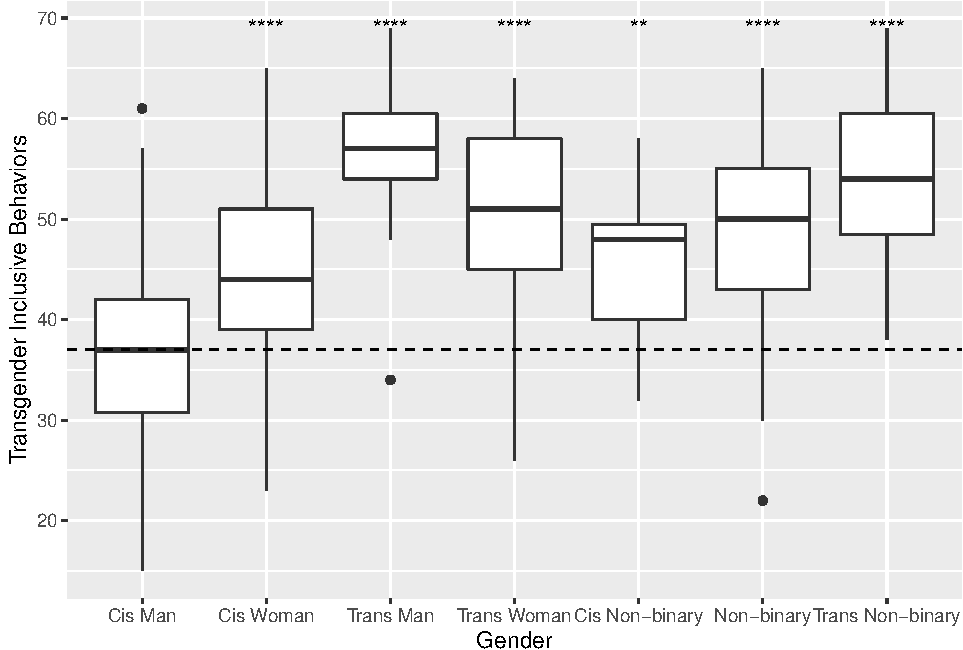
\includegraphics{thesis_files/figure-latex/unnamed-chunk-8-1.pdf}
\caption{\label{fig:unnamed-chunk-8}TIBS Scores by Gender}
\end{figure}
\hypertarget{pronouns-1}{%
\section{Pronouns}\label{pronouns-1}}

\hypertarget{comfort-sharing-pronouns}{%
\subsection{Comfort sharing pronouns}\label{comfort-sharing-pronouns}}

Items 1, 2, 3, 7, 8, and 9 touched on participant's comfort sharing their pronouns.
A one-way ANOVA found a significant effect of setting, gender, and pronouns on comfort sharing pronouns, \emph{F}(2, 1311) = 16.39, \emph{p} \textless{} 0.001. A post-hoc Tukey test found that generally, students are more comfortable sharing pronouns in class, (\emph{M} = 4.5, \emph{SD} = 0.98), and in non-academic settings at Reed, (\emph{M} = 4.43, \emph{SD} = 1.07), than they are in general, (\emph{M} = 4.14, \emph{SD} = 1.31). It also found that cisgender men, (\emph{M} = 4.65, \emph{SD} = 0.78), are more comfortable sharing their pronouns than trans men, (\emph{M} = 4.11, \emph{SD} = 1.24), trans women, (\emph{M} = 3.22, \emph{SD} = 1.51), and non-binary people, (\emph{M} = 3.66, \emph{SD} = 1.4).

One-way ANOVAs were used on each setting to elucidate effects of gender and pronoun within each setting. There were significant effects of gender in general, \emph{F}(6, 435) = 34.7, \emph{p} \textless{} 0.001, in non-academic settings at Reed, \emph{F}(6, 435) = 9.07, \emph{p} \textless{} 0.001, and in class, \emph{F}(6, 435) = 19.93, \emph{p} \textless{} 0.001. There were also significant effects of pronouns in general, \emph{F}(435, 435) = NA, \emph{p} = NA, in non-academic settings at Reed, \emph{F}(435, 435) = NA, \emph{p} = NA, and in class, \emph{F}(435, 435) = NA, \emph{p} = NA.

Post-hoc Tukey tests were used to compare gender groups within each setting. In general, cisgender men were more comfortable sharing their pronouns than trans women, non-binary people, and transgender non-binary people. In addition, cisgender women were more comfortable sharing their pronouns than trans men, trans women, cisgender non-binary people, non-binary people, and transgender non-binary people. \textbf{descriptives needed}

A one-way ANOVA was used to examine effects of social factors, gender, and pronouns on comfort sharing pronouns. Specifically, we examined whether people were more comfortable sharing their pronouns when a professor did so first, when someone else did first, and when the participant was with people of similar genders to their own. There were significant effects of social factor, \emph{F}(2, 1311) = 60.03, \emph{p} \textless{} 0.001, gender, \emph{F}(6, 1311) = 6.95, \emph{p} \textless{} 0.001, and pronouns, \emph{F}(6, 1311) = 15.66, \emph{p} \textless{} 0.001. A post-hoc Tukey test revealed that someone else saying their pronouns first makes the largest difference in making others comfortable sharing their pronouns. This is followed by the professor sharing their pronouns first, and finally the presence of people of similar genders to one's own.

\hypertarget{desire-to-share-pronouns}{%
\subsection{Desire to share pronouns}\label{desire-to-share-pronouns}}

Items 4, 5, and 6 touched on participant's desire to share their pronouns. A one-way ANOVA revealed significant effects of setting, \emph{F}(2, 1314) = 18.12, \emph{p} \textless{} 0.001, gender, \emph{F}(6, 1314) = 7.22, \emph{p} \textless{} 0.001, and pronouns \emph{F}(6, 1314) = 13.46, \emph{p} \textless{} 0.001. A post-hoc Tukey test revealed that people;s desire to share their pronouns is highest in classroom settings, followed by non-accade mic ettings atReed, and then lowest in general. Trans men reported a higher desire to share their pronouns than cisgender men, cisgender women, transgender women, cisgender non-binary people, and non-binary people. Transgender non-binary people also reported a higher desire to share their pronouns than cisgender men and non-binary people.

\hypertarget{concerns-about-sharing-pronouns}{%
\subsection{Concerns about sharing pronouns}\label{concerns-about-sharing-pronouns}}

Items 10, 11, and 12 touched on participant's concern that sharing their pronouns would draw unwanted attention to themselves. There were significant effects of setting, \emph{F}(2, 1314) = 27.49, \emph{p} \textless{} 0.001, gender \emph{F}(6, 1314) = 19.69, \emph{p} \textless{} 0.001, and pronouns, \emph{F}(6, 1314) = 23.44, \emph{p} \textless{} 0.001 on concern that sharing one's pronouns would draw unwanted attention to oneself. A post-hoc Tukey test revealed that participants were most concerned that sharing their pronouns would draw unwanted attention to them in general, followed by in non-academic settings at Reed, and least concerned in class.

\hypertarget{congruence-and-perception-of-pronouns}{%
\subsection{Congruence and perception of pronouns}\label{congruence-and-perception-of-pronouns}}

Items 13, 14, 15, 16, 17 and 18 touched upon participant's relationship to their pronouns, gender, and appearance. We ran one-way ANOVAs examing effects of gender and pronouns on each item with pos-hoc Tukey tests where relevant.

On item 13 (``I feel that the gender that people perceive me as and my pronouns are consistent with one another.''), there was a significant effect of gender, \emph{F}(6, 449) = 116.89, \emph{p} \textless{} 0.001. A post-hoc Tukey test found that cis men, (\emph{M} = 4.76, \emph{SD} = 0.6), experience higher consistency than trans men, (\emph{M} = 2.58, \emph{SD} = 1.62), trans women, (\emph{M} = 2.05, \emph{SD} = 1.1), cis non-binary people, (\emph{M} = 3.13, \emph{SD} = 1.77), non-binary people, (\emph{M} = 2.2, \emph{SD} = 1.27), and trans non-binary people, (\emph{M} = 1.85, \emph{SD} = 1.07). Cis women, (\emph{M} = 4.65, \emph{SD} = 0.85), also experience higher consistency than trans men, trans women, cis non-binary people, non-binary people, and trans non-binary people. Cis non-binary people also experience higher consistency than trans women. Finally, cis non-binary people experience higher consistency than non-binary people and trans non-binary people. There were no other significant differences between groups.

On item 14 (``I feel that my internal gender identity and pronouns are consistent with one another.''), there was a significant effect of gender, \emph{F}(6, 450) = 20, \emph{p} \textless{} 0.001. A post-hoc Tukey test found that cis men, (\emph{M} = 4.52, \emph{SD} = 0.89), and cis women, (\emph{M} = 4.53, \emph{SD} = 0.93), reported higher consistency than cis non-binary people, (\emph{M} = 3.07, \emph{SD} = 1.67), non-binary people, (\emph{M} = 3.11, \emph{SD} = 1.44), and trans non-binary people, (\emph{M} = 3.85, \emph{SD} = 1.34). Trans men, (\emph{M} = 4.5, \emph{SD} = 1.17), also reported higher consistency than cis non-binary people and non-binary people. Trans non-binary people also reported higher consistency than non-binary people. There were no other significant differences between groups.

On item 15 (``I feel that my pronouns represent my gender identity well.''), there was a significant effect of gender, \emph{F}(6, 450) = 14.67, \emph{p} \textless{} 0.001. A post-hoc Tukey test revealed that cis men, (\emph{M} = 4.35, \emph{SD} = 1.06), and cis women, (\emph{M} = 4.39, \emph{SD} = 1.07), reported higher representativeness than cis non-binary people, (\emph{M} = 3.07, \emph{SD} = 1.67), non-binary people, (\emph{M} = 3.11, \emph{SD} = 1.46), and trans non-binary people, (\emph{M} = 3.71, \emph{SD} = 1.3). Furthermore, trans men, (\emph{M} = 4.5, \emph{SD} = 0.9), reported higher representativeness than cis non-binary people and non-binary people. There were no other significant differences between groups.

On item 16 (``If I don't tell people what my pronouns are, they will misgender me.''), there was a significant effect of gender, \emph{F}(6, 450) = 75.91, \emph{p} \textless{} 0.001. A post-hoc Tukey test revealed that cis men, (\emph{M} = 1.95, \emph{SD} = 0.3), and cis women, (\emph{M} = 1.91, \emph{SD} = 0.47), are misgendered significantly less when they do not share their pronouns when compared to trans men, (\emph{M} = 3.75, \emph{SD} = 1.54), trans women, (\emph{M} = 4.1, \emph{SD} = 1.25), non-binary people, (\emph{M} = 3.32, \emph{SD} = 1.54), and trans non-binary people, (\emph{M} = 4.31, \emph{SD} = 1.17). Furthermore, cis non-binary, (\emph{M} = 2.47, \emph{SD} = 0.92), people are misgendered significantly less than trans men, trans women, and non-binary people. There were no other significant differences between groups.

On item 17 (``I don't need to tell people what my pronouns are, because they usually assume correctly.''), there was a significant effect of gender, \emph{F}(6, 449) = 78.45, \emph{p} \textless{} 0.001. A post-hoc Tukey test revealed that people correctly assume cis men's, (\emph{M} = 4.56, \emph{SD} = 0.95), and cis women's, (\emph{M} = 4.49, \emph{SD} = 1.09), pronouns more frequently when compared to trans men, (\emph{M} = 2.5, \emph{SD} = 1.17), trans women, (\emph{M} = 2.15, \emph{SD} = 1.04), cis non-binary people, (\emph{M} = 3.27, \emph{SD} = 1.58), non-binary people, (\emph{M} = 2.46, \emph{SD} = 1.2), and trans non-binary people, (\emph{M} = 1.92, \emph{SD} = 0.65). Cis non-binary people's pronouns are also assumed correctly more frequently than trans women's and trans non-binary people.

Finally, on item 18 (``I feel like people understand me better when I share my pronouns.''), there was a significant effect of gender, \emph{F}(6, 449) = 25.69, \emph{p} \textless{} 0.001. A post-hoc Tukey test revealed that trans men, (\emph{M} = 3.58, \emph{SD} = 1.56), trans women, (\emph{M} = 3.7, \emph{SD} = 1.22), non-binary people, (\emph{M} = 3.67, \emph{SD} = 1.22), and trans non-binary, (\emph{M} = 3.98, \emph{SD} = 1.12), people feel better understood when they share their pronouns when compared to cis men, (\emph{M} = 2.39, \emph{SD} = 0.93) and cis women, (\emph{M} = 2.54, \emph{SD} = 0.96).

\hypertarget{historical-experience-at-reed-college}{%
\subsection{Historical experience at Reed College}\label{historical-experience-at-reed-college}}

Item 19 (``In classes at Reed, professors usually introduce themselves with their pronouns'') asked students to report how frequently professors introduced themselves with their pronouns. A one-way ANOVA did not find a significant effect of gender, \emph{F}(6, 339) = 1.97, \emph{p} = 0.07, or major, \emph{F}(70, 339) = 1.26, \emph{p} = 0.1, on reported frequency of professors sharing their pronouns. However, when we only compared majors in which we had more than 5 students in, there were significant effects of both gender, \emph{F}(6, 311) = 2.12, \emph{p} = 0.05, and major, \emph{F}(20, 311) = 2.17, \emph{p} \textless{} 0.001.

Item 20 (``In classes at Reed, students usually introduce themselves with their pronouns'') asked students to report how often their peers introduced themselves with their pronouns. A one-way ANOVA revaled a significant effect of gender, \emph{F}(6, 339) = 3.67, \emph{p} \textless{} 0.001, but not major. When we only compared majors that we had more than 5 students in, there were significant effects of gender, \emph{F}(6, 311) = 2.12, \emph{p} = 0.05, and major, \emph{F}(20, 311) = 2.17, \emph{p} \textless{} 0.001.

\hypertarget{primary-component-analysis}{%
\subsection{Primary Component Analysis}\label{primary-component-analysis}}

Principal component analysis (PCA) was used on the pronoun and misgendering data. Using a Screen plot, we retained three components with an eigenvalue of 2.99, accounting for 52.1\% of the variance.
\begin{table}

\caption{\label{tab:unnamed-chunk-9}PCA Component Loadings}
\centering
\begin{tabular}[t]{l|r|r|r}
\hline
Item & Comp. 1 & Comp. 2 & Comp. 3\\
\hline
cis & -0.12 & -0.01 & 0.01\\
\hline
trans & 0.07 & 0.02 & 0.03\\
\hline
nonbinary & 0.11 & 0.01 & -0.02\\
\hline
gender.man & -0.04 & -0.03 & 0.03\\
\hline
gender.woman & -0.05 & 0.02 & 0.00\\
\hline
comfort\_general & -0.25 & 0.23 & 0.09\\
\hline
comfort\_reed & -0.11 & 0.23 & 0.00\\
\hline
comfort\_class & -0.15 & 0.22 & 0.04\\
\hline
desire\_general & 0.01 & 0.41 & 0.04\\
\hline
desire\_reed & 0.11 & 0.41 & -0.03\\
\hline
desire\_class & 0.06 & 0.41 & -0.03\\
\hline
comfort\_withsimilargenders & 0.27 & 0.21 & -0.03\\
\hline
comfort\_someoneelsefirst & 0.03 & 0.17 & 0.21\\
\hline
comfort\_proffirst & 0.03 & 0.19 & 0.20\\
\hline
attention\_general & 0.27 & -0.15 & 0.39\\
\hline
attention\_reed & 0.11 & -0.18 & 0.56\\
\hline
attention\_class & 0.16 & -0.14 & 0.38\\
\hline
gender\_perception\_consistent & -0.40 & 0.02 & 0.26\\
\hline
gender\_pronouns\_consistent & -0.15 & 0.21 & 0.25\\
\hline
pronouns\_represent & -0.14 & 0.22 & 0.27\\
\hline
willmisgender\_ifnopronouns & 0.30 & 0.08 & -0.06\\
\hline
assume\_pronouns\_correctly & -0.37 & -0.02 & 0.13\\
\hline
understand\_better & 0.20 & 0.19 & 0.02\\
\hline
profs\_share & -0.09 & 0.01 & -0.17\\
\hline
students\_share & -0.04 & 0.03 & -0.06\\
\hline
reed\_support & -0.19 & -0.09 & -0.06\\
\hline
misgendering\_freq & 0.30 & 0.02 & -0.08\\
\hline
misgendering\_stigma & 0.24 & 0.12 & 0.15\\
\hline
\end{tabular}
\end{table}
Inspection of the first component's loadings indicate that concern that consistency between others' perception of one's gender, others' assumptions about gender and pronouns, misgendering, and comfort when with people with similar genders to one's own are making significant contributions to the first component. Because these items are mainly concerned with the assumptions other people place on one's gender and pronouns, this component appears to be the amount that cisnormative assumptions about one's gender and appearance harms individuals.

Loadings from the second component encompasses one's desire to share one's pronouns in various settings, as well as how comfortable one feels doing so. Because the largest loading in the second component is one's desire to share pronouns, this seems to indicate one's readiness to share pronouns.

Loadings from the third component emphasize concern that sharing one's pronouns will draw unwanted attention, as well as when others---not necessarily of the same gender---share their pronouns first and how consistent and representative one's pronouns are with one's gender. This component appears to represent concern around sharing pronouns and fears of judgment or lack of understanding about one's pronouns.
\begin{figure}
\centering
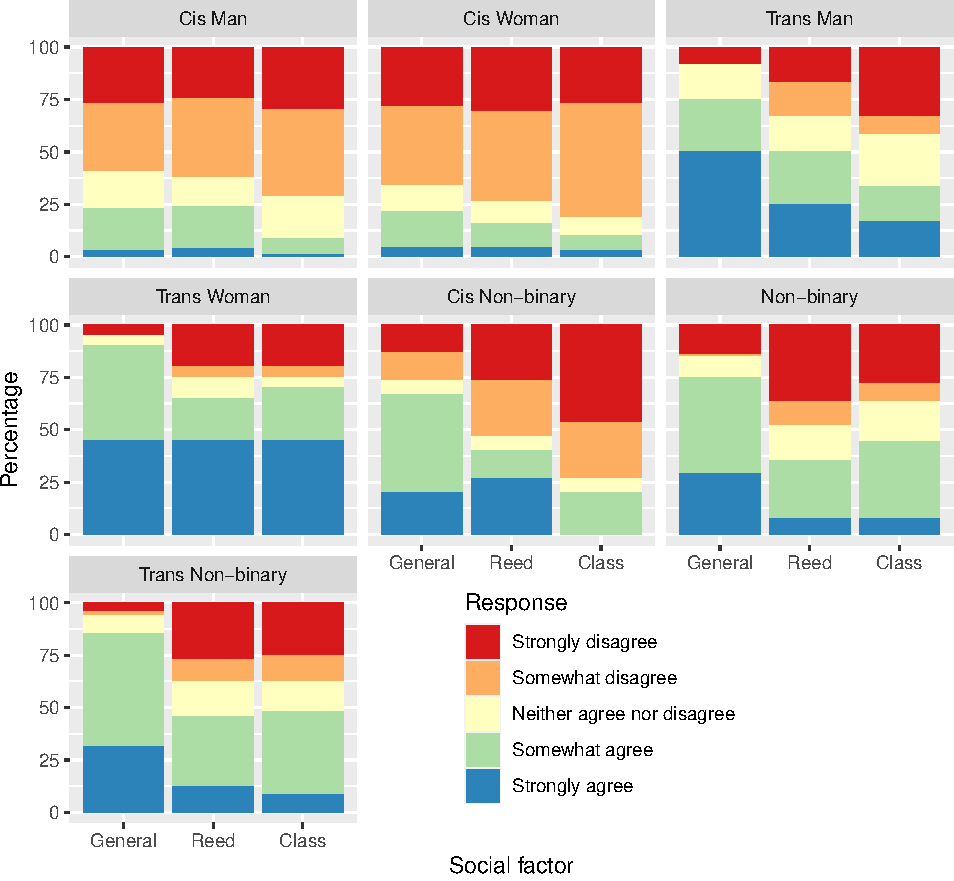
\includegraphics{thesis_files/figure-latex/unnamed-chunk-10-1.pdf}
\caption{\label{fig:unnamed-chunk-10}PCA Components 1 \& 2 by Gender}
\end{figure}
A one-way ANOVA demonstrated a significant effect of gender on the first component, \emph{F}(6, 391) = 226.3, \emph{p} \textless{} 0.001. A post-hoc Tukey test revealed that cisgender men, (\emph{M} = -2.72, \emph{SD} = 1.09), and women, (\emph{M} = -2.25, \emph{SD} = 1.37), are significantly less affected by cisnormativity than trans men, (\emph{M} = 3.28, \emph{SD} = 2.62), trans women, (\emph{M} = 4.32, \emph{SD} = 2), cisgender non-binary people, (\emph{M} = 0.64, \emph{SD} = 2.87), non-binary people, (\emph{M} = 3.4, \emph{SD} = 2.22), and transgender non-binary people, (\emph{M} = 4.56, \emph{SD} = 1.35). Cisgender non-binary people are also less affected than trans men, trans women, non-binary people, and transgender non-binary people. Trans non-binary people are also more affected than non-binary people.
\begin{figure}
\centering
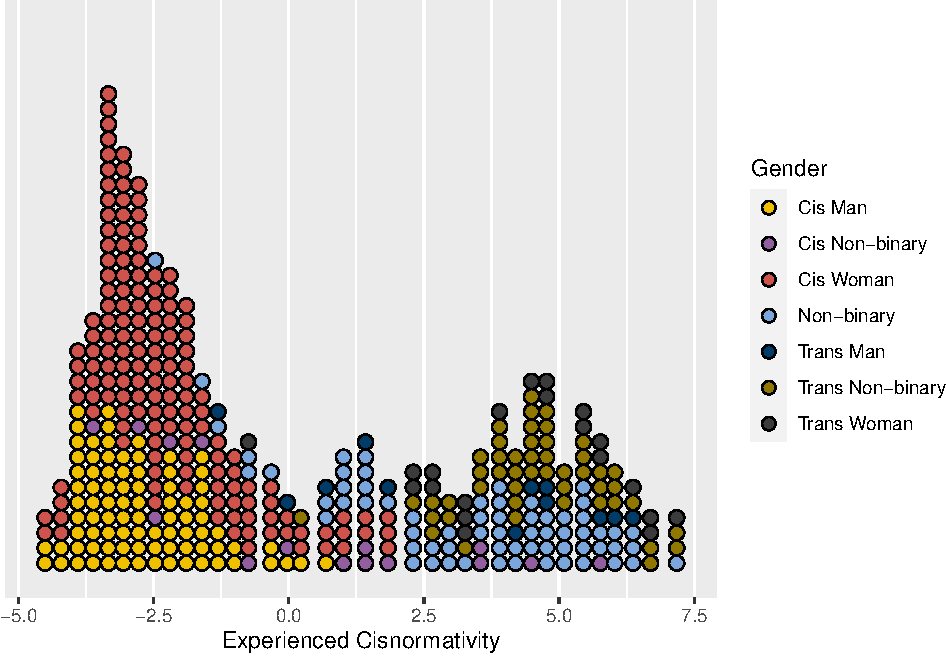
\includegraphics{thesis_files/figure-latex/unnamed-chunk-11-1.pdf}
\caption{\label{fig:unnamed-chunk-11}PCA Component 1 by Gender}
\end{figure}
Visualization of the first component indicated possible bimodality along the first component. Hartigan's dip test indicated that the distribution along the first component is unlikely to be unimodal, (\emph{D} = 0.032, \emph{p} = 0.006). This indicates that experiences with cisnormativity may be as bimodal. This indicates that cisgender and non-cisgender people may have significantly different experiences navigating the world as their gender.

Another one-way ANOVA demonstrated a significant effect of gender on the second component, \emph{F}(6, 391) = 6.15, \emph{p} \textless{} 0.001. A post-hoc Tukey test revealed that cisgender men, (\emph{M} = -2.72, \emph{SD} = 1.09), are less willing to share their pronouns than cisgender women, (\emph{M} = -2.25, \emph{SD} = 1.37) trans men, (\emph{M} = 3.28, \emph{SD} = 2.62), and non-binary people, (\emph{M} = 3.4, \emph{SD} = 2.22). Non-binary people are also more willing to share their pronouns than transgender women, (\emph{M} = 4.32, \emph{SD} = 2).

A final one-way ANOVA demonstrated a significant effect of gender on the third component, \emph{F}(6, 391) = 4.27, \emph{p} \textless{} 0.001. Non-binary people, (\emph{M} = 3.4, \emph{SD} = 2.22), are significantly less concerned that sharing their pronouns will draw unwanted attention than cisgender men, (\emph{M} = -2.72, \emph{SD} = 1.09), cisgender women, (\emph{M} = -2.25, \emph{SD} = 1.37), transgender men (\emph{M} = 3.28, \emph{SD} = 2.62), and transgender women (\emph{M} = 4.32, \emph{SD} = 2). There were no significant effects between any other groups.
\begin{figure}
\centering
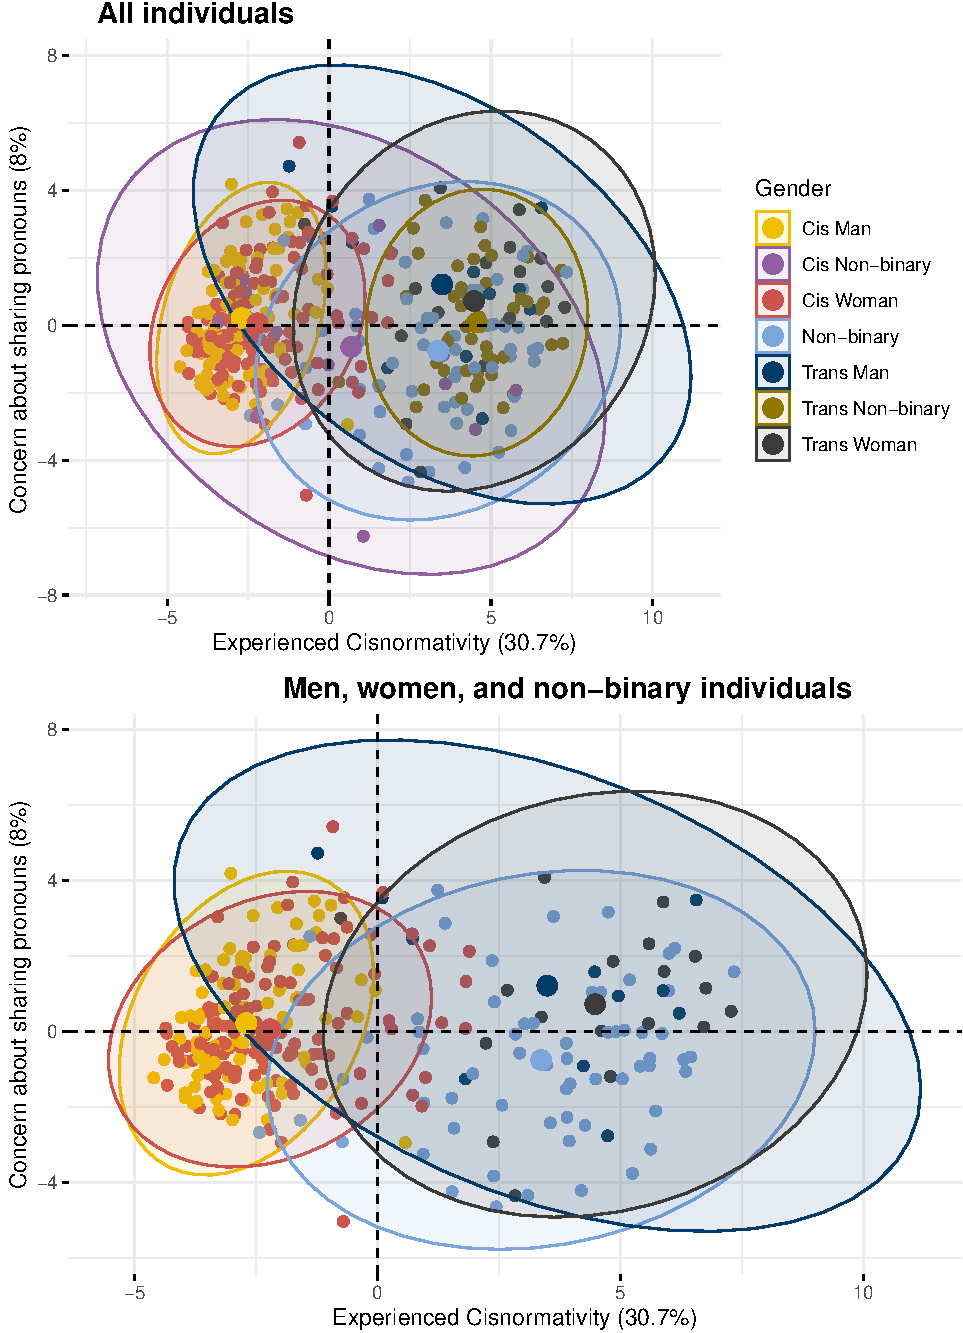
\includegraphics{thesis_files/figure-latex/unnamed-chunk-12-1.pdf}
\caption{\label{fig:unnamed-chunk-12}PCA Components 1 \& 3 by Gender}
\end{figure}
However, this may be due to the fact that this is the third component which only accounts for 7.8\% of the total variation. Visualization of the third component shows that there is considerable variation within groups.

\hypertarget{discussion}{%
\chapter{Discussion}\label{discussion}}

ooohhh my gooood oggggggg my ghoodododododododododod

\appendix

\hypertarget{appendix}{%
\chapter*{Appendix}\label{appendix}}
\addcontentsline{toc}{chapter}{Appendix}

\backmatter

\hypertarget{references}{%
\chapter*{References}\label{references}}
\addcontentsline{toc}{chapter}{References}

\markboth{References}{References}

\noindent

\setlength{\parindent}{-0.20in}
\setlength{\leftskip}{0.20in}
\setlength{\parskip}{8pt}

\hypertarget{refs}{}
\begin{cslreferences}
\leavevmode\hypertarget{ref-kattariDevelopmentValidationTransgender2018}{}%
Kattari, S. K., O'Connor, A. A., \& Kattari, L. (2018). Development and Validation of the Transgender Inclusive Behavior Scale (TIBS). \emph{Journal of Homosexuality}, \emph{65}(2), 181--196. \url{http://doi.org/10.1080/00918369.2017.1314160}

\leavevmode\hypertarget{ref-kozeeMeasuringTransgenderIndividuals2012}{}%
Kozee, H. B., Tylka, T. L., \& Bauerband, L. A. (2012). Measuring Transgender Individuals' Comfort With Gender Identity and Appearance: Development and Validation of the Transgender Congruence Scale. \emph{Psychology of Women Quarterly}, \emph{36}(2), 179--196. \url{http://doi.org/10.1177/0361684312442161}

\leavevmode\hypertarget{ref-mclemoreExperiencesMisgenderingIdentity2015}{}%
McLemore, K. A. (2015). Experiences with Misgendering: Identity Misclassification of Transgender Spectrum Individuals. \emph{Self and Identity}, \emph{14}(1), 51--74. \url{http://doi.org/10.1080/15298868.2014.950691}

\leavevmode\hypertarget{ref-nagoshiGenderDifferencesCorrelates2008}{}%
Nagoshi, J. L., Adams, K. A., Terrell, H. K., Hill, E. D., Brzuzy, S., \& Nagoshi, C. T. (2008). Gender Differences in Correlates of Homophobia and Transphobia. \emph{Sex Roles}, \emph{59}(7-8), 521--531. \url{http://doi.org/10.1007/s11199-008-9458-7}

\leavevmode\hypertarget{ref-reedcollegeinstitutionalresearchFactsReed2019}{}%
Reed College Institutional Research. (2019). Facts about Reed. https://www.reed.edu/ir/enrollment.html.

\leavevmode\hypertarget{ref-tateIntegratingStudyTransgender2014}{}%
Tate, C. C., Youssef, C. P., \& Bettergarcia, J. N. (2014). Integrating the Study of Transgender Spectrum and Cisgender Experiences of Self-Categorization from a Personality Perspective. \emph{Review of General Psychology}, \emph{18}(4), 302--312. \url{http://doi.org/10.1037/gpr0000019}
\end{cslreferences}

% Index?

\end{document}
